\documentclass{article}
\usepackage{amsmath}
\usepackage{titlesec}
\usepackage{graphicx}
\usepackage[margin=1in]{geometry}
\usepackage{hyperref}
\usepackage{float}

% Title, date, and author
\title{Exercise 3}
\author{Your Name, Collaborator's Name}
\date{\today}

\titleformat{\section}
  {\normalfont\normalsize\bfseries} % Format: font style, size, and weight
  {\thesection}{1em} % Label format and spacing
  {}
  \renewcommand{\thesubsection}{\thesection.\alph{subsection}}

\titleformat{\subsection}
  {\normalfont\small\bfseries} % Format: font style, size, and weight
  {\thesubsection}{1em} % Label format and spacing
  {}
\titleformat{\subsubsection}
  {\normalfont\small\bfseries} % Format: font style, size, and weight
  {\thesubsubsection}{1em} % Label format and spacing
  {}

\begin{document}
\begin{titlepage}
    \centering
    \vspace*{1in}
    
    {\Huge\bfseries Exercise 3\par}
    \vspace{1.5cm}
    {\Large \today\par}
    \vspace{1.5cm}
    {\Large\itshape Antonio Pampalone 23586519 \\ Giuseppe Pisante 23610012\\ Martina Raffaelli 23616907 \par}
    
    \vfill
    
\includegraphics[width=0.3\textwidth]{FAU-Logo.png}\par\vspace{1cm} % Adjust the width as needed
   
\end{titlepage}

\newpage
\small
\section{Finite difference approximation of the second derivative}
\subsection{fourth-order central finite-difference approximation}
We derive the fourth-order central finite-difference approximation for \( \frac{d^2f}{dx^2} \) using values of \( f \) at \( x_i \), \( x_{i-1} \), \( x_{i+1} \), \( x_{i-2} \), and \( x_{i+2} \), assuming a uniform grid spacing \( \Delta x \), as provided by the text.

We then expand \( f(x) \) at the neighboring points around \( x_i \) using Taylor series:

\begin{align*}
f(x_{i+1}) &= f(x_i) + f'(x_i)\Delta x + \frac{f''(x_i)}{2!}(\Delta x)^2 + \frac{f'''(x_i)}{3!}(\Delta x)^3 + \frac{f^{(4)}(x_i)}{4!}(\Delta x)^4 + \dots, \\
f(x_{i+2}) &= f(x_i) + 2f'(x_i)\Delta x + \frac{4f''(x_i)}{2!}(\Delta x)^2 + \frac{8f'''(x_i)}{3!}(\Delta x)^3 + \frac{16f^{(4)}(x_i)}{4!}(\Delta x)^4 + \dots, \\
f(x_{i-1}) &= f(x_i) - f'(x_i)\Delta x + \frac{f''(x_i)}{2!}(\Delta x)^2 - \frac{f'''(x_i)}{3!}(\Delta x)^3 + \frac{f^{(4)}(x_i)}{4!}(\Delta x)^4 - \dots, \\
f(x_{i-2}) &= f(x_i) - 2f'(x_i)\Delta x + \frac{4f''(x_i)}{2!}(\Delta x)^2 - \frac{8f'''(x_i)}{3!}(\Delta x)^3 + \frac{16f^{(4)}(x_i)}{4!}(\Delta x)^4 - \dots.
\end{align*}


As a further step, we add the symmetric spatial terms to cancel the odd derivatives:

\begin{align*}
f(x_{i+1}) + f(x_{i-1}) &= 2f(x_i) + \frac{2f''(x_i)}{2!}(\Delta x)^2 + \frac{2f^{(4)}(x_i)}{4!}(\Delta x)^4 + \dots, \\
f(x_{i+2}) + f(x_{i-2}) &= 2f(x_i) + \frac{8f''(x_i)}{2!}(\Delta x)^2 + \frac{32f^{(4)}(x_i)}{4!}(\Delta x)^4 + \dots.
\end{align*}


To approximate \( \frac{d^2f}{dx^2} \), we form a weighted sum of these terms:

\[
\frac{d^2f}{dx^2} = a [f(x_{i+1}) + f(x_{i-1})] + b [f(x_{i+2}) + f(x_{i-2})] + c f(x_i),
\]

where \( a, b, c \) are coefficients to be determined. \\
We substitute the Taylor expansions into \( S \):

\begin{align*}
  \frac{d^2f}{dx^2} &= 2a f(x_i) + 2b f(x_i) + c f(x_i) \\
  &\quad + \left( \frac{2a}{2!} (\Delta x)^2 + \frac{8b}{2!} (\Delta x)^2 \right) f''(x_i) \\
  &\quad + \left( \frac{2a}{4!} (\Delta x)^4 + \frac{32b}{4!} (\Delta x)^4 \right) f^{(4)}(x_i) + \dots
\end{align*}

Match coefficients for \( f(x_i), f''(x_i), \) and higher-order terms to ensure:
The coefficients are determined by matching terms in the Taylor series expansions:

\begin{enumerate}
  \item Coefficient of \( f(x_i) \):
  \[
  2a + 2b + c = 0
  \]
  \item Coefficient of \( f''(x_i) \): This should equal \( \frac{1}{(\Delta x)^2} \), so:
  \[
  a \cdot \frac{2(\Delta x)^2}{2!} + b \cdot \frac{8(\Delta x)^2}{2!} = \frac{1}{(\Delta x)^2}
  \]
  Simplifying:
  \[
  a + 4b = 6
  \]
  \item Coefficient of \( f^{(4)}(x_i) \): This term should be eliminated to ensure fourth-order accuracy:
  \[
  a \cdot \frac{2(\Delta x)^4}{4!} + b \cdot \frac{32(\Delta x)^4}{4!} = 0
  \]
  Simplifying:
  \[
  a + 16b = 0
  \]
\end{enumerate}


After solving the system of equations, the coefficients are:

\[
a = 16, \quad b = -1, \quad c = -30.
\]

We substitute these coefficients to get the fourth-order finite-difference approximation for \( \frac{d^2f}{dx^2} \):

\[
\frac{d^2f}{dx^2} \approx \frac{-f(x_{i+2}) + 16f(x_{i+1}) - 30f(x_i) + 16f(x_{i-1}) - f(x_{i-2})}{12 (\Delta x)^2}.
\]


\subsection{Second-order one-sided finite-difference approximation for \texorpdfstring{$\frac{\partial^2 u}{\partial x^2}$}{d2u/dx2}}
The backward second-order one-sided finite difference approximation for the second derivative \( \frac{d^2f}{dx^2} \) is derived as follows.
Expand \( f(x_{i-1}) \) and \( f(x_{i-2}) \) around \( x_i \) using Taylor series:
\[
f(x_{i-1}) = f(x_i) - f'(x_i) \Delta x + \frac{f''(x_i)}{2} (\Delta x)^2 - \frac{f^{(3)}(x_i)}{6} (\Delta x)^3 + O((\Delta x)^4),
\]
\[
f(x_{i-2}) = f(x_i) - 2f'(x_i) \Delta x + 2 \cdot \frac{f''(x_i)}{2} (\Delta x)^2 - \frac{2 \cdot f^{(3)}(x_i)}{6} (\Delta x)^3 + O((\Delta x)^4).
\]

We then subtract the first expansion from the second expansion:
\[
f(x_{i-2}) - 2f(x_{i-1}) + f(x_i) = \left( f(x_i) - 2f'(x_i) \Delta x + \frac{2 f''(x_i)}{2} (\Delta x)^2 + \dots \right)
- 2\left( f(x_i) - f'(x_i) \Delta x + \frac{f''(x_i)}{2} (\Delta x)^2 + \dots \right)
+ f(x_i).
\]

Simplifying:
\[
f(x_{i-2}) - 2f(x_{i-1}) + f(x_i) = \frac{f''(x_i)}{2} (\Delta x)^2 + O((\Delta x)^3).
\]

Thus, the backward second-order one-sided finite difference approximation for the second derivative is:
\[
\frac{d^2f}{dx^2} \approx \frac{f(x_i) - 2f(x_{i-1}) + f(x_{i-2})}{(\Delta x)^2}.
\]

This method is second-order accurate, with the leading error term proportional to \( O((\Delta x)^2) \).
It is important to note that this process can be applied to the forward difference scheme as well, with the same accuracy. In this case, the second derivative would be approximated as:
\[
\frac{d^2f}{dx^2} \approx \frac{f(x_{i+2}) - 2f(x_{i+1}) + f(x_i)}{(\Delta x)^2}.
\]

\subsection{Situations in which we need one-sided approximations}
Situations in which we need one-sided approximations include the discretization of convective terms, which are challenging to approximate with CDS due to instability. 
Another case could be the discretization of an hyperbolic problem, such as the example we studied in the stability lecture of the hyperbolic transport equation. In that case, BDS was way more stable than CDS.

\section{Finite difference approximation of the third and mixed derivatives}

\subsection{Second-order finite-difference approximation for \texorpdfstring{$\frac{\partial^3 \Psi}{\partial y^3}$}{d3Psi/dy3}}

We start by recalling the central difference formula for the second derivative:
\begin{equation}
\frac{\partial^2 \Psi}{\partial y^2} \approx \frac{\Psi(i+1) - 2\Psi(i) + \Psi(i-1)}{\Delta y^2}.
\end{equation}

To approximate the third derivative, we take the central difference of the second derivative:
\begin{equation}
\frac{\partial^3 \Psi}{\partial y^3} \approx \frac{\frac{\partial^2 \Psi}{\partial y^2}(i+1) - \frac{\partial^2 \Psi}{\partial y^2}(i-1)}{2\Delta y}.
\end{equation}

Substitute the expression for the second derivative into this formula. First, write $\frac{\partial^2 \Psi}{\partial y^2}(i+1)$ and $\frac{\partial^2 \Psi}{\partial y^2}(i-1)$ as:
\begin{align}
\frac{\partial^2 \Psi}{\partial y^2}(i+1) &\approx \frac{\Psi(i+2) - 2\Psi(i+1) + \Psi(i)}{\Delta y^2}, \\
\frac{\partial^2 \Psi}{\partial y^2}(i-1) &\approx \frac{\Psi(i) - 2\Psi(i-1) + \Psi(i-2)}{\Delta y^2}.
\end{align}

Substituting these into the expression for the third derivative:
\begin{equation}
\frac{\partial^3 \Psi}{\partial y^3} \approx \frac{\frac{\Psi(i+2) - 2\Psi(i+1) + \Psi(i)}{\Delta y^2} - \frac{\Psi(i) - 2\Psi(i-1) + \Psi(i-2)}{\Delta y^2}}{2\Delta y}.
\end{equation}

Combine the terms in the numerator:
\begin{equation}
\frac{\partial^3 \Psi}{\partial y^3} \approx \frac{\Psi(i+2) - 2\Psi(i+1) + \Psi(i) - \Psi(i) + 2\Psi(i-1) - \Psi(i-2)}{2\Delta y^3}.
\end{equation}

We simplify further, and we get the following result:
\begin{equation}
\frac{\partial^3 \Psi}{\partial y^3} \approx \frac{\Psi(i+2) - 2\Psi(i+1) + 2\Psi(i-1) - \Psi(i-2)}{2\Delta y^3}.
\end{equation}


\subsection{Second-order finite-difference approximation for \texorpdfstring{$\frac{\partial^2 \Psi}{\partial y \partial x}$}{d2Psi/dy dx}}
To derive the finite-difference approximation for the mixed derivative $\frac{\partial^2\Psi}{\partial x\partial y}$, we'll follow a similar step-by-step process as we did for the higher-order derivatives with respect to $y$.
First, let's review the central difference formula for the partial derivative $\frac{\partial\Psi}{\partial y}$:
\begin{equation}
\frac{\partial\Psi}{\partial y} \approx \frac{\Psi(i+1,j) - \Psi(i-1,j)}{2\Delta y}
\end{equation}
Now, to get the mixed derivative $\frac{\partial^2\Psi}{\partial x\partial y}$, we need to differentiate this first derivative expression with respect to $x$:
\begin{align}
\frac{\partial^2\Psi}{\partial x\partial y} &\approx \frac{\frac{\partial\Psi}{\partial y}(i+1,j+1) - \frac{\partial\Psi}{\partial y}(i-1,j+1) - \frac{\partial\Psi}{\partial y}(i+1,j-1) + \frac{\partial\Psi}{\partial y}(i-1,j-1)}{4\Delta x\Delta y}
\end{align}
Substituting the central difference formula for $\frac{\partial\Psi}{\partial y}$, we get:
\begin{align}
\frac{\partial^2\Psi}{\partial x\partial y} &\approx \frac{(\Psi(i+1,j+1) - \Psi(i-1,j+1)) - (\Psi(i+1,j-1) - \Psi(i-1,j-1))}{4\Delta x\Delta y}
\end{align}
Simplifying the expression, the final second-order finite-difference approximation for the mixed derivative $\frac{\partial^2\Psi}{\partial x\partial y}$ is:
\begin{equation}
\frac{\partial^2\Psi}{\partial x\partial y} \approx \frac{\Psi(i+1,j+1) - \Psi(i-1,j+1) - \Psi(i+1,j-1) + \Psi(i-1,j-1)}{4\Delta x\Delta y}
\end{equation}

\section{Steady temperature distribution of an alluminium bar}

\subsection{Non-dimensional form of the heat equation}

The time-dependent heat equation in 1D is:

\[
\rho c_p \frac{\partial T}{\partial t} = \lambda \frac{\partial^2 T}{\partial x^2}
\]

In this formulation, we have replaced the temperature \(T\) with the function \(u(x, t)\).

\[
\frac{\partial u}{\partial t} = \alpha \frac{\partial^2 u}{\partial x^2}
\]

where \(\alpha\) is the thermal diffusivity defined as:

\[
\alpha = \frac{\lambda}{c \rho} 
\]

To derive the non-dimensional form of the heat equation we have to introduce the dimensionless variables \(\hat{x}\), \(\hat{t}\),
and \(\hat{u}\), respectively, for position, time and temperature:

\[
\hat{x} = \frac{x}{L^*}, \quad \hat{t} = \frac{t}{T^*}, \quad \hat{u}(\hat{x}, \hat{t}) = \frac{u(x, t)}{U^*}
\]

Since the characteristic length, time, and temperature are \( L^* \), \( T^* \), and \( U^* \), respectively, with dimensions:

\[
[L^*] = L, \quad [T^*] = T, \quad [U^*] = U.
\]

The choice for the characteristic length is \( L^* = l \), the length of the rod, in this way, while \( x \) is in the range 
\( 0 < x < l \), \(\hat{x}\) is in the range \( 0 < \hat{x} < 1 \). In the following passages taken from the source \cite{HeatEquation}, we have:

\[
\frac{\partial u}{\partial t} = \frac{\partial \hat{u}}{\partial \hat{t}} \cdot \frac{U^*}{T^*} = \frac{U^*}{T^*} \frac{\partial \hat{u}}{\partial \hat{t}},
\]
\[
\frac{\partial u}{\partial x} = \frac{\partial \hat{u}}{\partial \hat{x}} \cdot \frac{U^*}{L^*} = \frac{U^*}{L^*} \frac{\partial \hat{u}}{\partial \hat{x}},
\]
\[
\frac{\partial^2 u}{\partial x^2} = \frac{U^*}{L^*} \cdot \frac{1}{L^*} \frac{\partial^2 \hat{u}}{\partial \hat{x}^2} = \frac{U^*}{L^2} \frac{\partial^2 \hat{u}}{\partial \hat{x}^2}.
\]

Substituting these into the heat equation gives:
\[
\frac{U^*}{T^*} \frac{\partial \hat{u}}{\partial \hat{t}} = \alpha \frac{U^*}{L^2} \frac{\partial^2 \hat{u}}{\partial \hat{x}^2}.
\]

To make the PDE simpler, we choose for the characteristic time \( T^* = \frac{L^2}{\alpha}\), so that the equation becomes:
\[
\frac{\partial \hat{u}}{\partial \hat{t}} = \frac{\partial^2 \hat{u}}{\partial \hat{x}^2}
\]

The most important non-dimensional number for this problem is the Fourier number wich characterizes 
the ratio of conductive heat transfer to thermal storage and is used to analyze heat conduction in this context.

\[
Fo = \frac{\lambda t}{\rho c_p L^2}
\]

\subsection{Dimensional form of the equation for the numerical solution}

For our numerical solution we want to use the dimensional form of the equation because in this way, we can maintain physical units while 
controlling stability numerically. This approach allows us to define a grid in terms of the effective length $L$ and the time interval 
$\Delta t$, thereby maintaining physical units. The values of $\rho$, $c_p$, $\lambda$, and $q$ can be directly substituted into 
the discretized equation in their dimensional form, and the boundary conditions can be applied directly. Furthermore, once the numerical 
solution is computed, the temperature at all nodes $T_i^n$ is obtained directly in Kelvin, preserving dimensional consistency. 
While non-dimensionalization may simplify some analyses, it is not strictly necessary for straightforward numerical implementation.

\subsection{Discretization using a second-order central differende scheme in space}

At the boundaries, the Central difference scheme cannot be directly applied because one or both adjacent points fall outside the domain. 
To address this, we use the Forward Difference Scheme at the first boundary point and the Backward Difference Scheme at the last boundary point. 
This ensures that the second derivative is computed for all points in the domain. The formulas used are as follows:

1. Central Difference Scheme for interior points:
\[
f''(x_i) \approx \frac{f(x_{i+1}) - 2f(x_i) + f(x_{i-1})}{\Delta x^2}
\]

2. Forward Difference Scheme at the first boundary point:
\[
f''(x_0) \approx \frac{f(x_2) - 2f(x_1) + f(x_0)}{\Delta x^2}
\]

3. Backward Difference Scheme at the last boundary point:
\[
f''(x_{N-1}) \approx \frac{f(x_{N-1}) - 2f(x_{N-2}) + f(x_{N-3})}{\Delta x^2}
\]

\subsection{Verify the correctness of the implementation}

Looking at the plot, the functions \( f(x) = \sin(x) \) and \( f(x) = x^3 \) verify the expected second-order convergence of the central 
difference scheme. In contrast, the functions at the bottom show very small errors that slightly increase as the grid spacing becomes finer.
This increase in error is due to numerical precision limitations rather than an issue with the method itself. For functions like \( f(x) = x \) 
and \( f(x) = x^2 \), the analytical second derivatives are either zero or constant. As the grid spacing \( \Delta x \) becomes very small,
 the central difference scheme involves subtracting nearly equal numbers, which amplifies round-off errors, leading to the observed increase
in error for finer grids.


\begin{figure}[h!]
  \centering
  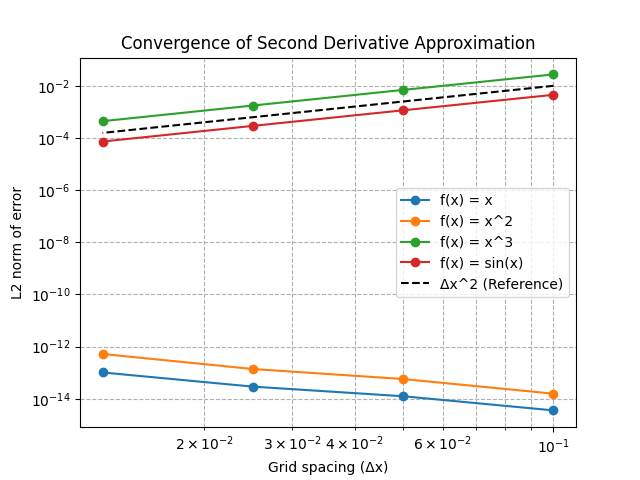
\includegraphics[width=0.5\textwidth]{Figure_4.png}
  \caption{Convergence of second derivative approximation}
  \label{fig: Convergence of second derivative approximation}
\end{figure}

\subsection{Stationary temperature distribution}

The attached file \texttt{1D\_Heat.py} from our repository \cite{GitHubRepo} contains the Python code which should be executed to obtain 
the numerical solution of the 1D Heat equation respectively in the cases of stationary temperature distribution (with and without heat source) 
and unsteady evolution of temperature. The result depicted in the graph illustrates the steady-state temperature distribution along an alluminium
bar. The temperature distribution is linear between the imposed boundary conditions, reflecting the absence of any internal heat source.

\begin{figure}[h!]
  \centering
  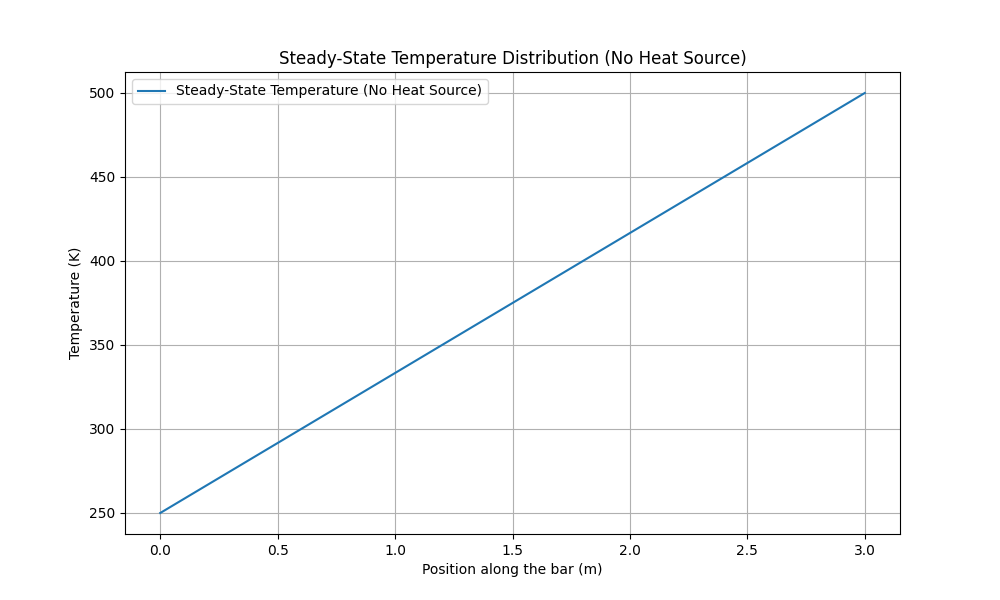
\includegraphics[width=0.5\textwidth]{Figure_1.png}
  \caption{Stationary temperature distribution}
  \label{fig: Stationary temperature distribution}
\end{figure}

\subsection{Stationary temperature distribution with a homogeneus heat source}

The result depicted in this graph represents the steady-state temperature distribution with a homogeneous heat source. Unlike the case with no
heat source, the temperature distribution here is non-linear, with a distinct peak near the center of the bar. This indicates that internal heat
generation significantly affects the temperature distribution. In contrast, when no heat source is present, the temperature distribution is linear,
as the heat transfer occurs solely due to conduction.

\begin{figure}[H]
  \centering
  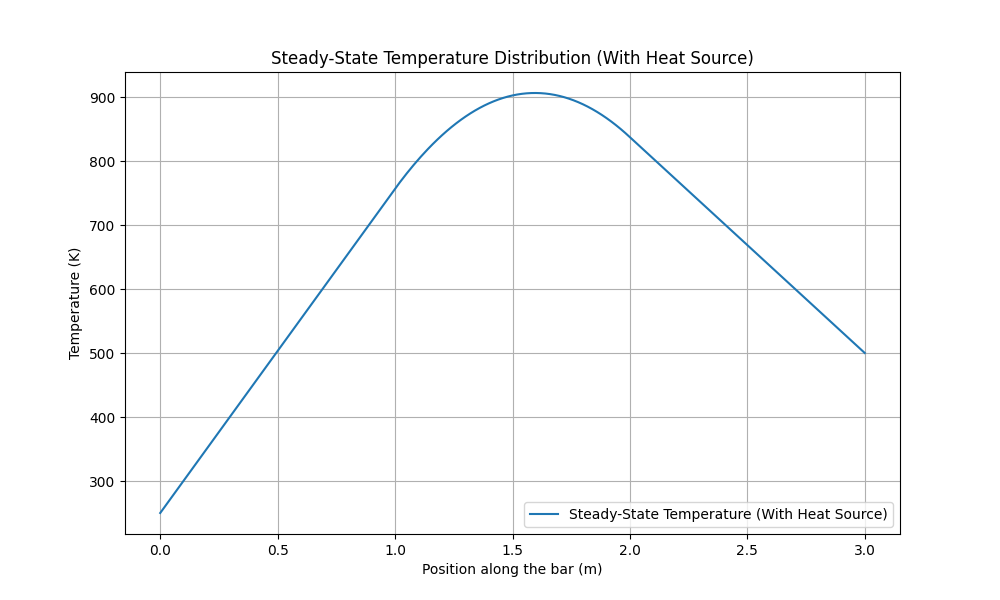
\includegraphics[width=0.5\textwidth]{Figure_2.png}
  \caption{Stationary temperature distribution with a homogeneus heat source}
  \label{fig: Stationary temperature distribution with a homogeneus heat source}
\end{figure}

\subsection{Unsteady evolution of temperature}

The result depicted in this graph represents the unsteady evolution of temperature of the bar. Initially, the temperature is a linear profile 
likely corresponding to a steady-state condition with no heat source effect. As time progresses, the temperature rises across the bar due to 
the heat generated internally. The curves demonstrate how heat gradually accumulates in the material, with the most pronounced rise occurring 
in the center of the bar.

\begin{figure}[H]
  \centering
  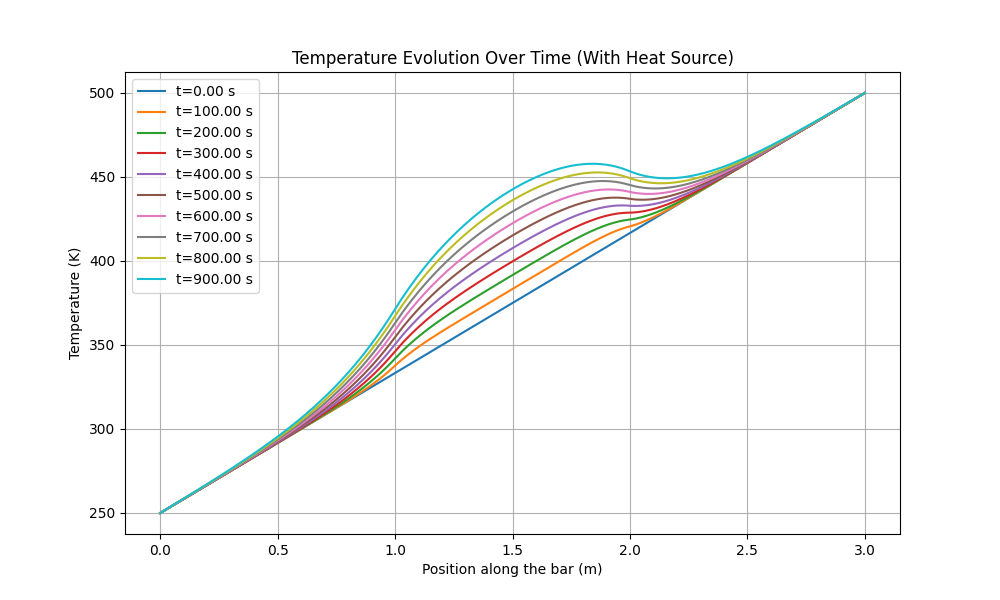
\includegraphics[width=0.5\textwidth]{Figure_3.png}
  \caption{Unsteady evolution of temperature}
  \label{fig: Unsteady evolution of temperature}
\end{figure}

\begin{thebibliography}{9}
  \bibitem{GitHubRepo}
  \textit{CFD Repository},\\
  Available at: \url{https://github.com/GiuseppePisante/CFD.git}
  
  \bibitem{GitHubCopilot}
  \textit{GitHub Copilot},\\
  GitHub. Available at: \url{https://github.com/features/copilot}
  
  \bibitem{HeatEquation}
  MIT OpenCourseWare,\\
  \textit{Heat Equation Notes}, 2006,\\
  Available at: \url{https://ocw.mit.edu/courses/18-303-linear-partial-differential-equations-fall-2006/d11b374a85c3fde55ec971fe587f8a50_heateqni.pdf},\\
\end{thebibliography}

\end{document}